\documentclass[11pt]{article}
\usepackage[margin=1in]{geometry}
\usepackage[T1]{fontenc}
\usepackage{lmodern}
\usepackage{amsmath,amssymb}
\usepackage{booktabs}
\usepackage{siunitx}
\usepackage{graphicx}
\usepackage{xcolor}
\usepackage[numbers,sort&compress]{natbib}
\usepackage{hyperref}
\usepackage{cleveref}
\hypersetup{colorlinks=true,linkcolor=blue!50!black,citecolor=blue!50!black,urlcolor=blue!50!black}
\sisetup{group-minimum-digits=4}
\emergencystretch=2em

% GENERATED by figures/make_figures.py from results/*.json -- do not edit
\newif\ifprovisional
\provisionaltrue
\newcommand{\benchMode}{dev}
\newcommand{\gpuName}{NVIDIA GeForce RTX 3070 Laptop GPU}
\newcommand{\copyBW}{361}
\newcommand{\bestTwoName}{cupy-cuda-c/fused-inplace-lean}
\newcommand{\bestTwoN}{4096}
\newcommand{\bestTwoMs}{27.05}
\newcommand{\bestTwoMpts}{620}
\newcommand{\bestTwoRoof}{99}
\newcommand{\bestTwoCopy}{52}
\newcommand{\bestTwoSpec}{42}
\newcommand{\bestTwoFFTGpts}{9.9}
\newcommand{\bestTwoFFTshare}{70}
\newcommand{\bestTwoRoofMs}{26.87}
\newcommand{\bestTwoFFTMs}{18.87}
\newcommand{\ladderTwoN}{2048}
\newcommand{\ladderTwoName}{cupy-cuda-c/fused-inplace-graph}
\newcommand{\ladderTwoRoof}{95}
\newcommand{\speedupTwoEager}{2.8}
\newcommand{\speedupTwoTextbook}{5.4}
\newcommand{\cpuTwoN}{1024}
\newcommand{\cpuTwoGPUName}{cupy-cuda-c/fused-inplace-graph}
\newcommand{\speedupTwoCPU}{26}
\newcommand{\fpRatioTwoN}{2048}
\newcommand{\fpRatioTwo}{6.3}
\newcommand{\bestThreeName}{cupy-cuda-c/fused-inplace-lean}
\newcommand{\bestThreeN}{192}
\newcommand{\bestThreeMs}{22.41}
\newcommand{\bestThreeMpts}{316}
\newcommand{\bestThreeRoof}{103}
\newcommand{\bestThreeCopy}{57}
\newcommand{\bestThreeSpec}{46}
\newcommand{\bestThreeFFTGpts}{10.1}
\newcommand{\bestThreeFFTshare}{68}
\newcommand{\bestThreeRoofMs}{23.00}
\newcommand{\bestThreeFFTMs}{15.34}
\newcommand{\ladderThreeN}{128}
\newcommand{\ladderThreeName}{cupy-cuda-c/fused-inplace-graph}
\newcommand{\ladderThreeRoof}{104}
\newcommand{\speedupThreeEager}{3.7}
\newcommand{\speedupThreeTextbook}{6.6}
\newcommand{\cpuThreeN}{64}
\newcommand{\cpuThreeGPUName}{cupy-cuda-c/fused-inplace-lean}
\newcommand{\speedupThreeCPU}{42}
\newcommand{\rotN}{128}
\newcommand{\rotOverBasd}{1.24}
\newcommand{\fpRatioThreeN}{128}
\newcommand{\fpRatioThree}{5.6}
\newcommand{\perfTableRows}{2D $2048^2$ & \texttt{torch-eager/c2c-textbook} & 20 & 34.89 & 120 & 44 & 12 & 22 \\
2D $2048^2$ & \texttt{torch-eager/r2c-textbook} & 20 & 19.82 & 212 & 77 & 21 & 38 \\
2D $2048^2$ & \texttt{torch-eager/r2c-minfft} & 16 & 18.06 & 232 & 70 & 19 & 34 \\
2D $2048^2$ & \texttt{torch-compile/inductor} & 16 & 10.76 & 390 & 117 & 32 & 57 \\
2D $2048^2$ & \texttt{cupy/elementwise} & 16 & 10.12 & 414 & 124 & 34 & 60 \\
2D $2048^2$ & \texttt{warp/fused} & 16 & 9.11 & 461 & 138 & 38 & 67 \\
2D $2048^2$ & \texttt{triton/fused} & 16 & 9.07 & 462 & 139 & 38 & 67 \\
2D $2048^2$ & \texttt{cupy-cuda-c/fused-inplace} & 16 & 6.46 & 649 & 195 & 54 & 95 \\
2D $2048^2$ & \texttt{cupy-cuda-c/fused-inplace-graph} & 16 & 6.42 & 653 & 196 & 54 & 95 \\
\midrule
3D $128^3$ & \texttt{torch-eager/c2c-textbook} & 36 & 43.27 & 48 & 35 & 10 & 18 \\
3D $128^3$ & \texttt{torch-eager/r2c-minfft} & 32 & 24.13 & 87 & 56 & 16 & 28 \\
3D $128^3$ & \texttt{torch-eager/r2c-textbook} & 36 & 23.96 & 88 & 63 & 17 & 32 \\
3D $128^3$ & \texttt{torch-compile/inductor} & 32 & 10.95 & 192 & 125 & 34 & 63 \\
3D $128^3$ & \texttt{cupy/elementwise} & 32 & 9.34 & 224 & 146 & 40 & 74 \\
3D $128^3$ & \texttt{triton/fused} & 32 & 8.74 & 240 & 156 & 43 & 79 \\
3D $128^3$ & \texttt{warp/fused} & 32 & 8.71 & 241 & 156 & 43 & 79 \\
3D $128^3$ & \texttt{cupy-cuda-c/fused-inplace-lean} & 32 & 6.77 & 310 & 201 & 56 & 102 \\
3D $128^3$ & \texttt{cupy-cuda-c/fused-inplace} & 32 & 6.65 & 315 & 205 & 57 & 103 \\
3D $128^3$ & \texttt{cupy-cuda-c/fused-inplace-graph} & 32 & 6.60 & 318 & 207 & 57 & 104 \\}
\newcommand{\tgvTwoErrSixtyFour}{\num{3.1e-15}}
\newcommand{\tgvTwoErrThirtyTwo}{\num{7.0e-6}}
\newcommand{\tgvTwoNVariants}{11}
\newcommand{\rkOrder}{4.07}
\newcommand{\ifrkOrder}{3.99}
\newcommand{\spatialErrMin}{\num{6.1e-11}}
\newcommand{\spatialNMax}{64}
\newcommand{\spatialNRef}{192}
\newcommand{\aggErrSixtyFour}{\num{1.3e-15}}
\newcommand{\aggErrThirtyTwo}{\num{8.3e-7}}
\newcommand{\aggN}{64}
\newcommand{\tgvN}{256}
\newcommand{\tgvPeak}{0.01291}
\newcommand{\tgvPeakTime}{8.90}
\newcommand{\tgvRefPeak}{0.01286}
\newcommand{\tgvRefPeakTime}{8.97}
\newcommand{\tgvPeakErr}{0.43}
\newcommand{\tgvMaxErr}{5.94}
\newcommand{\tgvSteps}{4075}
\newcommand{\tgvWall}{476}
\newcommand{\tgvTableRows}{$64^3$ & 0.01340 & 9.20 & +4.18 & 14.91 & 1167 \\
$128^3$ & 0.01376 & 8.90 & +7.01 & 9.48 & 2109 \\
$192^3$ & 0.01298 & 8.85 & +0.98 & 3.09 & 3048 \\
$256^3$ & 0.01291 & 8.90 & +0.43 & 5.94 & 4075 \\}
\newcommand{\twoSlope}{-3.83}
\newcommand{\twoN}{512}
\newcommand{\twoFit}{15\le k\le 50}
\newcommand{\threeSlope}{-1.48}
\newcommand{\threeN}{192}
\newcommand{\threeRe}{80}
\newcommand{\threeKeta}{1.48}
\newcommand{\threeFit}{3\le k\le 8}

\providecommand{\aggErrSixtyFour}{n/a}
\providecommand{\aggErrThirtyTwo}{n/a}
\providecommand{\aggN}{n/a}
\providecommand{\benchMode}{n/a}
\providecommand{\bestThreeFFTshare}{n/a}
\providecommand{\bestThreeMs}{n/a}
\providecommand{\bestThreeN}{n/a}
\providecommand{\bestThreeRoof}{n/a}
\providecommand{\bestTwoMs}{n/a}
\providecommand{\bestTwoN}{n/a}
\providecommand{\bestTwoName}{n/a}
\providecommand{\bestTwoRoof}{n/a}
\providecommand{\copyBW}{n/a}
\providecommand{\cpuTwoN}{n/a}
\providecommand{\fpRatioTwo}{n/a}
\providecommand{\fpRatioTwoN}{n/a}
\providecommand{\gpuName}{n/a}
\providecommand{\ifrkOrder}{n/a}
\providecommand{\ladderTwoN}{n/a}
\providecommand{\ladderTwoName}{n/a}
\providecommand{\rkOrder}{n/a}
\providecommand{\rotN}{n/a}
\providecommand{\rotOverBasd}{n/a}
\providecommand{\spatialErrMin}{n/a}
\providecommand{\spatialNMax}{n/a}
\providecommand{\spatialNRef}{n/a}
\providecommand{\speedupTwoCPU}{n/a}
\providecommand{\speedupTwoEager}{n/a}
\providecommand{\speedupTwoTextbook}{n/a}
\providecommand{\tgvMaxErr}{n/a}
\providecommand{\tgvN}{n/a}
\providecommand{\tgvPeak}{n/a}
\providecommand{\tgvPeakErr}{n/a}
\providecommand{\tgvPeakTime}{n/a}
\providecommand{\tgvRefPeak}{n/a}
\providecommand{\tgvRefPeakTime}{n/a}
\providecommand{\tgvTableRows}{n/a}
\providecommand{\tgvTwoErrSixtyFour}{n/a}
\providecommand{\tgvTwoErrThirtyTwo}{n/a}
\providecommand{\tgvTwoNVariants}{n/a}
\providecommand{\threeFit}{n/a}
\providecommand{\threeKeta}{n/a}
\providecommand{\threeN}{n/a}
\providecommand{\threeRe}{n/a}
\providecommand{\threeSlope}{n/a}
\providecommand{\twoFit}{n/a}
\providecommand{\twoN}{n/a}
\providecommand{\twoSlope}{n/a}
\providecommand{\perfTableRows}{}
\providecommand{\tgvTableRows}{}

\title{Spectral DNS of turbulence near the FFT roofline from Python}
\author{Walid Hemati\\Independent researcher}
\date{}

\begin{document}
\maketitle

\ifprovisional
\begin{center}
\fcolorbox{red}{red!8}{\parbox{0.9\linewidth}{\centering\bfseries\color{red!70!black}
PROVISIONAL NUMBERS --- performance figures and tables in this version come from a development
run on a shared GPU (\texttt{bench/run.py --\benchMode}) and are not publishable. Validation
results are final.}}
\end{center}
\fi

\begin{abstract}
Pseudo-spectral direct numerical simulation (DNS) of incompressible turbulence spends almost all
of its time in fast Fourier transforms. On a GPU those FFTs are memory-bound, so a time step has a
hard lower bound: the number of transforms times the time of a standalone cuFFT call, plus the
bytes the remaining pointwise work must move. We call this bound the \emph{FFT roofline}.
\texttt{pyspectral} is a Python package that solves the 2D vorticity equation and the 3D
Navier--Stokes equations in rotational form on a periodic box. It uses 2/3-rule dealiasing,
integrating-factor RK4 and CFL-adaptive time steps. Eleven interchangeable backend variants span an
optimisation ladder: NumPy/SciPy, eager PyTorch, \texttt{torch.compile}, CuPy elementwise
kernels, NVIDIA Warp, Triton and hand-written CUDA C compiled at run time. Every backend is
validated against a NumPy oracle. The 2D Taylor--Green vortex is reproduced to
\tgvTwoErrSixtyFour{} in double precision. RK4 converges at order \rkOrder{}, and the spatial
error decays exponentially in the resolution. The 3D Taylor--Green vortex at $Re=1600$ on a
$\tgvN^3$ grid reaches peak dissipation \tgvPeak{} at $t=\tgvPeakTime$; the $512^3$ reference
gives \tgvRefPeak{} at $t=\tgvRefPeakTime$. Three measures bring a step close to the FFT
roofline: Basdevant's reformulation (4 instead of 5 FFTs per stage in 2D, 8 instead of 9 in
3D), one fused kernel on each side of the transforms, and in-place batched cuFFT plans. On an
\gpuName{} the fastest variant (\texttt{\bestTwoName}) advances a $\bestTwoN^2$ grid in
\bestTwoMs{}\,ms per RK4 step, \bestTwoRoof\,\% of the FFT roofline, and a $\bestThreeN^3$ grid
in \bestThreeMs{}\,ms (\bestThreeRoof\,\%).
\end{abstract}

\section{Introduction}

Fourier pseudo-spectral methods have been the reference discretisation for DNS of homogeneous
turbulence since the work of Orszag and Patterson~\cite{orszag1971aliasing,patterson1971spectral}
and Rogallo~\cite{rogallo1981numerical}. They are still the method of choice for the largest
simulations~\cite{yokokawa2002tflops,ishihara2009study,ravikumar2019gpu,yeung2025gpu}. Each time
step is a sequence of forward and inverse multi-dimensional FFTs, joined by cheap pointwise
operations in physical and spectral space. On modern GPUs large FFTs are limited by memory
bandwidth, not arithmetic. A pseudo-spectral code therefore cannot run faster than the FFT
library allows. Its efficiency is set by two things: how many FFTs it needs per step, and how
little extra memory traffic surrounds them.

This paper asks whether that hardware limit can be reached from Python. Mortensen and
Langtangen~\cite{mortensen2016high} showed that a pure-Python/NumPy pseudo-spectral solver on
CPUs can nearly match a C++ implementation. Dedalus~\cite{burns2020dedalus} is a general Python
spectral framework. Neither study measures a single GPU against its own roofline. We do that,
following the roofline methodology of Williams et al.~\cite{williams2009roofline}. The
ceiling is not peak FLOP/s or raw bandwidth. It is the measured time of the standalone cuFFT
calls the algorithm cannot avoid. Our contributions are:
\begin{itemize}
\item A pseudo-spectral Navier--Stokes solver, \texttt{pyspectral}: 2D vorticity form and 3D
  rotational form with Leray projection, 2/3-rule (or phase-shift) dealiasing, Lawson
  integrating-factor RK4~\cite{lawson1967generalized}, CFL-adaptive steps, and constant-power
  forcing. Eleven backend variants share one interface and one test suite.
\item An FFT-count-minimal formulation following Basdevant~\cite{basdevant1983technical}: 4
  real-to-complex transforms per RK stage in 2D and 8 in 3D, with a fused schedule. Each stage
  runs exactly two pointwise kernels, the transforms are batched and in place, and the integrating
  factor comes from a separable table.
\item An \emph{FFT roofline} for pseudo-spectral steps. It combines the measured standalone cuFFT
  time for the exact batched transforms of a stage with a minimal pointwise-traffic model. We
  report every backend as a fraction of it.
\item Validation against exact solutions and against the $512^3$ reference DNS of the
  Taylor--Green vortex at $Re=1600$~\cite{wang2013high,vanrees2011comparison}, plus forced 2D
  and 3D spectra.
\end{itemize}

\section{Background and related work}

\paragraph{Pseudo-spectral DNS.} In the Fourier--Galerkin/collocation method the nonlinear term is
evaluated in physical space, so quadratic products alias. Orszag's 2/3 rule removes aliasing
exactly for quadratic terms by truncating $|k_i|\ge N/3$~\cite{orszag1971aliasing}. Phase shifts
with spherical truncation~\cite{patterson1971spectral,rogallo1981numerical} keep more modes at the
price of extra transforms or randomisation. Textbook treatments are given by Canuto et
al.~\cite{canuto1988spectral,canuto2006spectral}. Basdevant~\cite{basdevant1983technical}
introduced formulations of the nonlinear term that need fewer transforms. Exponential and
integrating-factor integrators treat the stiff linear term exactly~\cite{lawson1967generalized,
cox2002exponential}. Record DNS runs pushed Fourier methods to $4096^3$ on the Earth
Simulator~\cite{yokokawa2002tflops,ishihara2009study}. More recent work runs them on thousands of
GPUs~\cite{ravikumar2019gpu,yeung2025gpu}. Those codes target aggregate throughput on
supercomputers. Our claim is narrower: per-GPU hardware efficiency from Python.

\paragraph{Python for spectral DNS.} Mortensen and Langtangen~\cite{mortensen2016high} report that
their pure-Python solver is about 30\,\% slower than their own C++ port in serial runs. On a Blue
Gene/P their optimised version matched C++ across processor counts. Dedalus~\cite{burns2020dedalus}
generalises spectral methods to many equations and bases. Neither targets GPUs. On the GPU side,
Python now offers several kernel-generation routes: PyTorch~\cite{paszke2019pytorch} and its
compiler~\cite{ansel2024pytorch2}, Triton~\cite{tillet2019triton}, CuPy~\cite{okuta2017cupy}
and NVIDIA Warp~\cite{macklin2022warp}. All of them can call cuFFT~\cite{cufft}. CPU FFTs use
pocketfft through SciPy~\cite{virtanen2020scipy,harris2020array}, in the role FFTW plays in
compiled codes~\cite{frigo2005fftw}.

\section{Method}

\subsection{Equations}
We solve the incompressible Navier--Stokes equations on $[0,2\pi)^d$ with integer wavenumbers
$\mathbf{k}$. In 2D we evolve the vorticity $\omega=\partial_x v-\partial_y u$,
\begin{equation}
\partial_t\omega + \nabla\cdot(\mathbf{u}\,\omega) = \nu\nabla^2\omega - \alpha\,\omega + f,
\qquad \hat\psi = \hat\omega/k^2,\quad \hat u = \mathrm{i}k_y\hat\psi,\quad
\hat v=-\mathrm{i}k_x\hat\psi .
\end{equation}
In 3D we evolve the velocity in rotational form,
\begin{equation}
\partial_t\hat{\mathbf u} = \mathsf P(\mathbf k)\,\widehat{\mathbf u\times\boldsymbol\omega}
 - \nu k^2\hat{\mathbf u} + \hat{\mathbf f},\qquad
 \mathsf P_{ij}=\delta_{ij}-k_ik_j/k^2,
\end{equation}
where the Leray projector $\mathsf P$ absorbs the pressure and the gradient of the kinetic
energy.

\subsection{Fewer transforms per stage}
The textbook 2D advective form $\mathbf u\cdot\nabla\omega$ needs four inverse transforms
($u,v,\omega_x,\omega_y$) and one forward transform. The 3D rotational form needs six inverse
($\mathbf u,\boldsymbol\omega$) and three forward. Following Basdevant~\cite{basdevant1983technical},
for divergence-free $\mathbf u$ we use the identity (checked by direct expansion and
numerically in our tests)
\begin{equation}
\nabla\cdot(\mathbf u\,\omega) = \partial_x\partial_y\,(v^2-u^2) + (\partial_x^2-\partial_y^2)\,(uv),
\end{equation}
which needs only the inverse transforms of $u,v$ and the forward transforms of $v^2-u^2$ and
$uv$: 4 FFTs. In 3D we write the nonlinear term in divergence form with the traceless stress
$T_{ij}=u_iu_j-\tfrac13|\mathbf u|^2\delta_{ij}$. The trace is a gradient and the projection
removes it. Since $T_{33}=-T_{11}-T_{22}$, the term
$\hat N_i=-\mathrm i\,\mathsf P_{ij}k_l\hat T_{jl}$ needs 3 inverse and 5 forward transforms
(8 instead of 9). With the 2/3 rule all products are computed exactly on the retained modes,
so the rotational and the divergence form give identical results up to round-off. Our
tests confirm this at the $10^{-16}$ level.

\subsection{Dealiasing, time integration and forcing}
We keep modes with $3|k_i|<N$ in every direction (cubic 2/3 truncation). The NumPy and eager
PyTorch backends also offer random phase shifts with spherical truncation
$|\mathbf k|<\sqrt2N/3$. The shift is redrawn each step and moved by half a grid cell between
the first and the second pair of RK stages, after Rogallo~\cite{rogallo1981numerical}. The
linear operator
\begin{equation}
L(\mathbf k) = -\nu k^2 - \alpha\,[k\le k_\alpha] + A\,[k_{\rm lo}\le k\le k_{\rm hi}]
\end{equation}
combines viscosity, linear drag (uniform if $k_\alpha=\infty$, otherwise acting on large scales
only) and band-limited linear forcing. The forcing is a spectral variant of the linear forcing
of Lundgren~\cite{lundgren2003linearly,rosales2005linear}. A constant-power controller resets
$A=P/(2E_{\rm band})$ every few steps. With $E=e^{L\Delta t}$ and $E_{1/2}=e^{L\Delta t/2}$, the
Lawson integrating-factor RK4~\cite{lawson1967generalized} reads
\begin{align}
k_1&=N(u_n), & k_2&=N\!\big(E_{1/2}(u_n+\tfrac{\Delta t}{2}k_1)\big), \nonumber\\
k_3&=N\!\big(E_{1/2}u_n+\tfrac{\Delta t}{2}k_2\big), & k_4&=N\!\big(Eu_n+\Delta t\,E_{1/2}k_3\big),
\nonumber\\
u_{n+1}&=Eu_n+\tfrac{\Delta t}{6}\big(Ek_1+2E_{1/2}(k_2+k_3)+k_4\big). &&
\end{align}
It integrates the linear term exactly and needs one accumulator besides the state. The step
size follows $\Delta t=C\,\Delta x/\sum_i\max|u_i|$ with $C=0.5$, re-evaluated every 10 steps.

\section{Implementation: the optimisation ladder}
\label{sec:impl}

All backends implement the same \texttt{SpectralSolver} interface and are listed in a registry
(\cref{tab:perf}). The NumPy/SciPy backend is a direct transcription of the equations. It is the
correctness oracle and runs in CI. The GPU backends form a ladder:
\begin{description}
\item[torch-eager] ports the NumPy code to \texttt{torch.fft}. The variants use complex-to-complex
  transforms on the full spectrum (\texttt{c2c-textbook}), real-to-complex transforms
  (\texttt{r2c-textbook}), and the minimal FFT count (\texttt{r2c-minfft}). Every arithmetic
  operation launches its own kernel and allocates a temporary.
\item[torch-compile] writes the two pointwise phases as plain PyTorch on real views of the
  complex buffers. TorchInductor compiles them into fused Triton kernels. Stage coefficients and
  $\Delta t$ come from a device tensor, so adaptive steps never trigger recompilation.
\item[cupy] fuses each phase into one \texttt{ElementwiseKernel} and calls the
  SciPy-compatible \texttt{cupyx.scipy.fft} API (cached plans, out-of-place).
\item[warp, triton] use hand-written fused kernels in NVIDIA Warp and Triton. They run on
  preallocated torch buffers with \texttt{torch.fft} transforms written into fixed output
  buffers. The forward-FFT output doubles as the next inverse-FFT input.
\item[cupy-cuda-c] is the hand-written reference: CUDA C compiled at run time by NVRTC through
  CuPy's \texttt{RawModule}, with batched \emph{in-place} cuFFT plans (\texttt{cufftPlanMany}
  with padded real layout) created through CuPy's low-level plan interface. The \texttt{lean}
  variant loops over single-field plans to save memory. The \texttt{graph} variant captures one
  time step in a CUDA graph.
\end{description}

\paragraph{Fused schedule.} One RK stage of the fused backends is
\emph{C2R (batched, in place) $\to$ physical kernel $\to$ R2C (batched, in place) $\to$ spectral
kernel}. The physical kernel reads $u,v$ (3D: $\mathbf u$) and writes the products in place over
them. The spectral kernel reads the transformed products, assembles $\hat N$, applies the
dealiasing mask and the projection, and performs the IF-RK4 stage update on the state and the
accumulator. It then writes the next stage's FFT inputs: the streamfunction velocities in 2D,
$\hat{\mathbf u}$ (and $\hat{\boldsymbol\omega}$ for the rotational form) in 3D, already scaled
by $N^{-d}$ for the unnormalised cuFFT inverse. No separate ``pre'' kernel exists. Viscous
factors cost no transcendental functions because
$e^{-\nu k^2\theta\Delta t}=t_\theta[|k_x|]\,t_\theta[|k_y|]\,t_\theta[|k_z|]$ separates into a
1D table, with drag and band forcing applied as two scalar factors. This matters in fp64, where
\texttt{exp} is expensive on consumer GPUs. The memory footprint is the state, the accumulator
and $\max(n_{\rm inv},n_{\rm fwd})$ work fields: 4 spectral fields in 2D, 11 in 3D.

\paragraph{FFT roofline and traffic model.} Let $t_{\rm FFT}$ be the measured time of the
batched C2R plus R2C transforms of one stage. We use the faster of in-place CuPy plans and
out-of-place \texttt{torch.fft}, timed standalone on identical shapes. Let $B$ be the minimal
pointwise traffic per step. The physical kernel reads the $n_{\rm inv}$ inverse outputs and
writes the $n_{\rm fwd}$ products. The spectral kernel reads the $n_{\rm fwd}$ transformed
products and the $c$ state components, writes $n_{\rm inv}$ next inputs, and reads and writes the
accumulator ($7c$ field transfers per step). The FFT-roofline step time is
\begin{equation}
T_{\rm roof} = 4\,t_{\rm FFT} + B/B_{\rm copy},\qquad B_{\rm copy}=\SI{361}{GB/s},
\label{eq:roof}
\end{equation}
where $B_{\rm copy}$ is the device-to-device copy bandwidth measured for the whole suite (the
datasheet value is \SI{448}{GB/s}). We report $T_{\rm roof}/T_{\rm step}$ as ``\% of FFT
roofline''. For the conventional bandwidth view we also count each FFT as one read and one
write of its data, which is a lower bound because real 2D/3D FFTs take several passes. Adding
$B$ gives an effective bandwidth that can only be under-, never over-estimated. Throughput is
given in Mpts/s, grid points advanced by one full RK4 step per second.

\section{Validation}

\paragraph{Exact solutions and convergence.} The 2D Taylor--Green vortex
$\omega=2\sin x\sin y$ is a steady Euler solution, so it decays as $e^{-2\nu t}$. Integrating
factors make IF-RK4 exact for it. All \tgvTwoNVariants{} variants reproduce it to
\tgvTwoErrSixtyFour{} (fp64) and \tgvTwoErrThirtyTwo{} (fp32). With the viscous term treated
explicitly, classical RK4 converges at order \rkOrder{} (\cref{fig:conv}). For a nonlinear,
non-band-limited flow, IF-RK4 self-convergence gives order \ifrkOrder{}. The spatial error
against an $N=\spatialNRef$ solution decays exponentially, to \spatialErrMin{} at
$N=\spatialNMax$. Every GPU variant matches the fp64 NumPy oracle across \aggN{} cases (2D/3D,
both 3D forms, with drag, forcing, a changed forcing amplitude and a changed $\Delta t$) to
\aggErrSixtyFour{} in fp64 and \aggErrThirtyTwo{} in fp32. Further tests check inviscid energy
conservation, the 2D energy budget $\mathrm dE/\mathrm dt=-2\nu Z$, a divergence-free velocity,
and agreement of phase-shift with 2/3-rule dealiasing.

\begin{figure}[!htb]
\centering
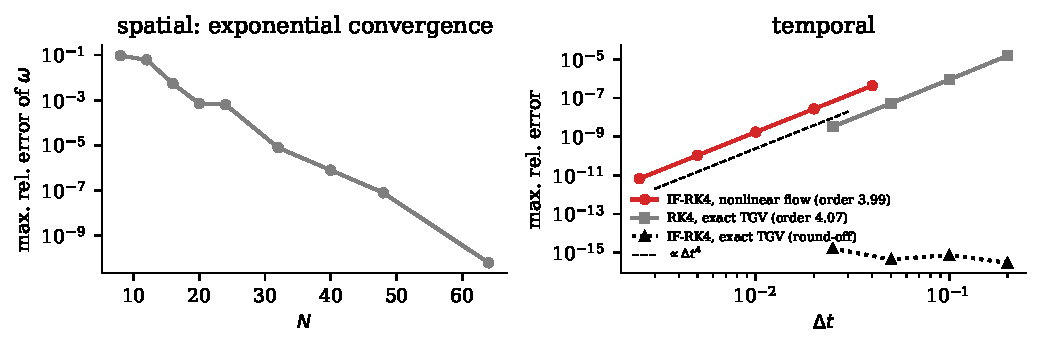
\includegraphics[width=\linewidth]{../figures/fig_conv2d.pdf}
\caption{Left: spectral convergence in $N$ for a smooth 2D flow (error against
$N=\spatialNRef$). Right: temporal convergence. Classical RK4 on the exact TGV decay, IF-RK4
self-convergence on a nonlinear flow, and IF-RK4 on the TGV, which is exact to round-off.}
\label{fig:conv}
\end{figure}

\paragraph{3D Taylor--Green vortex at $Re=1600$.} The initial condition is
$u=\sin x\cos y\cos z$, $v=-\cos x\sin y\cos z$, $w=0$ with $\nu=1/1600$, integrated to
$t=20$.
This is the benchmark of the high-order CFD workshops~\cite{wang2013high,debonis2013solutions},
originally studied by Brachet et al.~\cite{brachet1983small}. We compare the dissipation rate
$\varepsilon=2\nu Z$ with the $512^3$ pseudo-spectral reference distributed for workshop case
C3.5. Its documentation attributes the data to a dealiased pseudo-spectral code from
Universit\'e catholique de Louvain and cites van Rees et al.~\cite{vanrees2011comparison} for an
independent spectral convergence study. The comparison is in \cref{tab:tgv,fig:tgv}. At
$\tgvN^3$ the peak is \tgvPeak{} at $t=\tgvPeakTime$, against \tgvRefPeak{} at
$t=\tgvRefPeakTime$ in the reference (\tgvPeakErr\,\% difference). The largest deviation over
$t\in[0,20]$ is \tgvMaxErr\,\% of the peak value. It occurs after the peak, during the
breakdown into small-scale turbulence. Coarser grids over-predict the peak, as expected for
under-resolved Galerkin truncations, where energy piles up near the cutoff. The peak error
falls monotonically with $N$ (\cref{tab:tgv}). The post-peak deviation does not: it is smaller
at $192^3$ than at $256^3$. Possible causes are the remaining resolution
gap to the $512^3$ reference, single precision (which can break the flow's discrete symmetries
earlier than a double-precision run), and the different time integrator of the reference
(low-storage RK3). We have not separated these effects.

\begin{table}[!htb]
\centering
\caption{3D Taylor--Green vortex at $Re=1600$ (fp32, \texttt{cupy-cuda-c}, CFL 0.5) against
the $512^3$ reference (peak \tgvRefPeak{} at $t=\tgvRefPeakTime$).}
\label{tab:tgv}
\begin{tabular}{lrrrrr}
\toprule
grid & peak $\varepsilon$ & $t_{\rm peak}$ & peak error [\%] & max $|\Delta\varepsilon|/\varepsilon_{\max}$ [\%] & steps\\
\midrule
\tgvTableRows
\bottomrule
\end{tabular}
\end{table}

\begin{figure}[!htb]
\centering
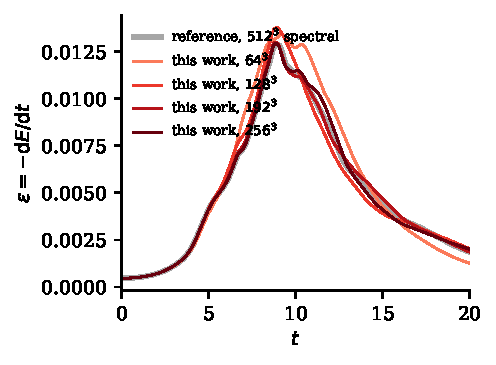
\includegraphics[width=0.6\linewidth]{../figures/fig_tgv3d.pdf}
\caption{Kinetic-energy dissipation rate of the Taylor--Green vortex at $Re=1600$ against the
$512^3$ spectral reference.}
\label{fig:tgv}
\end{figure}

\paragraph{Forced turbulence.} Constant-power band forcing gives statistically stationary
turbulence (\cref{fig:spectra}). In 2D ($N=\twoN$, forcing at $k\approx4$, drag on $k\le2.5$) the
enstrophy-cascade range has $E(k)\sim k^{\twoSlope}$ for $\twoFit$. That is steeper than
Kraichnan's $k^{-3}$~\cite{kraichnan1967inertial,boffetta2012two}, as is common at this
modest scale separation with large-scale friction. In 3D ($N=\threeN$, $k_{\max}\eta=\threeKeta$)
the Taylor-scale Reynolds number is only $Re_\lambda=\threeRe$. The compensated spectrum
therefore shows only a short plateau just above the forcing scale, followed by the dissipation
range, and no extended $k^{-5/3}$ range~\cite{kolmogorov1941local}. The local slope over
$\threeFit$ is $\threeSlope$. Both runs serve as end-to-end tests of the forcing,
drag and diagnostics machinery. They are not converged turbulence statistics.

\begin{figure}[!htb]
\centering
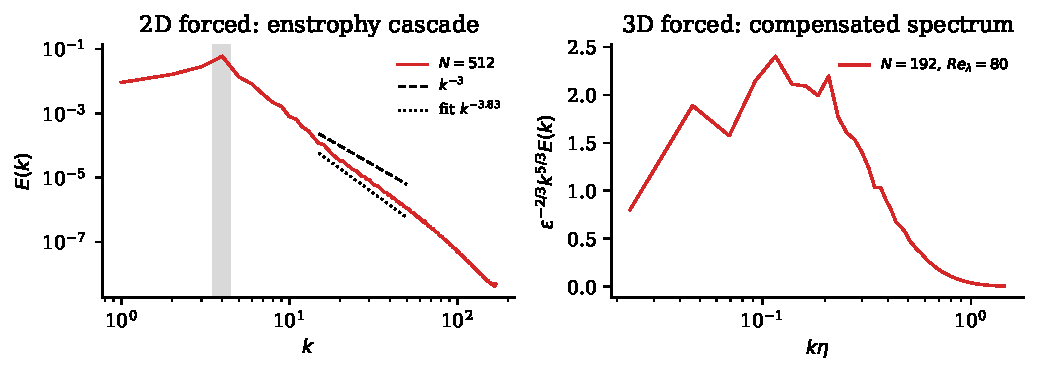
\includegraphics[width=\linewidth]{../figures/fig_spectra.pdf}
\caption{Time-averaged energy spectra of forced turbulence. Left: 2D (grey band: forcing). Right:
3D, compensated by $\varepsilon^{-2/3}k^{5/3}$.}
\label{fig:spectra}
\end{figure}

\section{Performance}

All performance numbers come from \texttt{bench/run.py} on an \gpuName{} (GA104, 40 SMs,
8\,GB GDDR6, datasheet bandwidth \SI{448}{GB/s}, measured copy bandwidth \copyBW\,GB/s).
We report the median of 5 repeats, each lasting at least \SI{0.5}{s} (fewer in the provisional
dev run), after a warm-up that covers JIT compilation, plan creation and autotuning.

\begin{figure}[!htb]
\centering
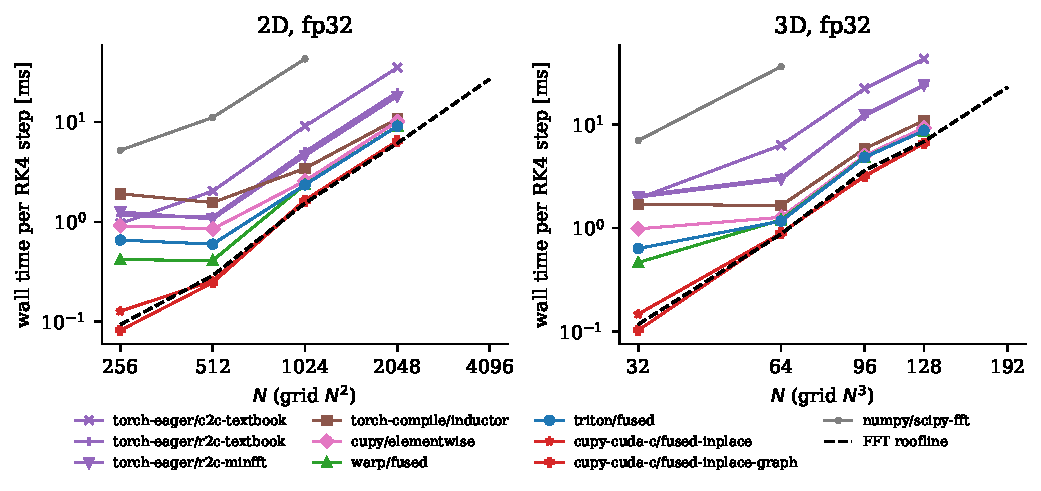
\includegraphics[width=\linewidth]{../figures/fig_scaling.pdf}
\caption{Wall time per RK4 step against grid size (fp32), with the FFT roofline
\eqref{eq:roof} (dashed).}
\label{fig:scaling}
\end{figure}

\begin{figure}[!htb]
\centering
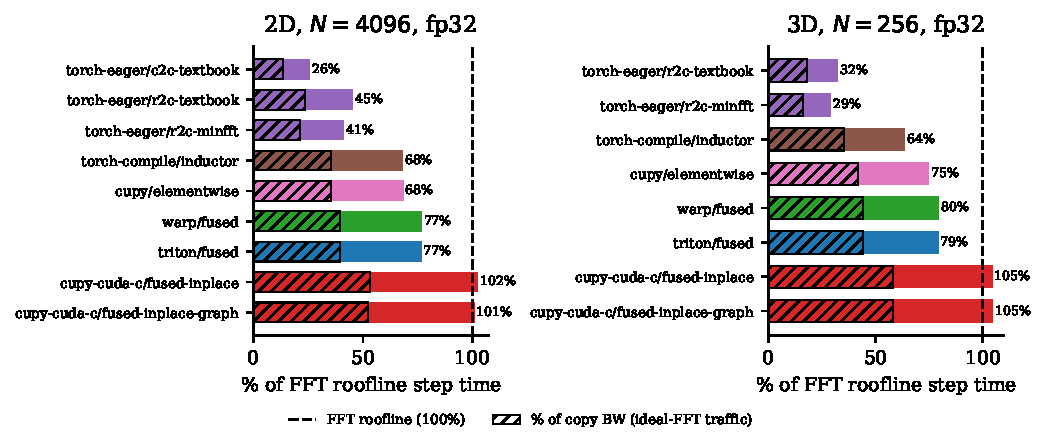
\includegraphics[width=\linewidth]{../figures/fig_roofline.pdf}
\caption{Fraction of the FFT roofline reached by each variant at the largest grid (solid). The
hatched bars show effective bandwidth as a percentage of \SI{361}{GB/s} under the ideal
single-pass FFT traffic model. Dashed line: the roofline.}
\label{fig:roof}
\end{figure}

\begin{table}[!htb]
\centering
\footnotesize
\caption{Step times at the largest grids (fp32). ``FFT'' is the number of real FFTs per RK4 step;
``GB/s'' and ``\% copy'' use the ideal traffic model; ``\% roof'' is $T_{\rm roof}/T_{\rm step}$.}
\label{tab:perf}
\begin{tabular}{llrrrrrr}
\toprule
grid & variant & FFT & ms/step & Mpts/s & GB/s & \% copy & \% roof\\
\midrule
\perfTableRows
\bottomrule
\end{tabular}
\end{table}

\paragraph{The ladder.} \Cref{fig:scaling,fig:roof,tab:perf} show the progression. Eager PyTorch
pays for every intermediate array. At $\ladderTwoN^2$, the largest 2D grid on which every rung
ran, the fastest variant (\texttt{\ladderTwoName}) is \speedupTwoEager$\times$ faster than eager PyTorch with the same FFT count, and
\speedupTwoTextbook$\times$ faster than the complex-to-complex textbook version. Against the
multithreaded NumPy/SciPy reference on 16 CPU threads at $N=\cpuTwoN$ (2D) the speed-up is
\speedupTwoCPU$\times$. Fusing the pointwise phases into one kernel each (Inductor, CuPy, Warp,
Triton) removes most of the gap. What remains is mostly the transforms. For identical shapes,
the out-of-place \texttt{torch.fft} and \texttt{cupyx.scipy.fft} calls are measurably slower
than in-place batched cuFFT plans; both timings are stored with the results. At the largest grids the
fastest variants reach \bestTwoRoof\,\% of the FFT roofline in 2D (\texttt{\bestTwoName},
$\bestTwoN^2$) and \bestThreeRoof\,\% in 3D (\texttt{\bestThreeName}, $\bestThreeN^3$), where
the FFTs alone take \bestThreeFFTshare\,\% of the step. At $\rotN^3$ the rotational form (9 FFTs) takes \rotOverBasd$\times$ the step time of the
Basdevant form (8 FFTs) in the CUDA C backend. CUDA graphs pay off only on small grids, where launch
latency dominates.

\paragraph{Precision.} On this consumer GPU, double-precision arithmetic runs at a small fraction
of single-precision throughput. Double-precision FFTs therefore become compute-bound: at
$\fpRatioTwoN^2$ an fp64 step of the CUDA C backend takes \fpRatioTwo$\times$ as long as an fp32
step, much more than the $2\times$ that the doubled byte count alone would cause. Production DNS on such hardware is therefore done in fp32. The
Taylor--Green results above use fp32 and agree with the fp64 reference to the plotting
accuracy.



\section{Discussion}

At large $N$ the pointwise work is almost free once fused, so the FFT library is the ceiling.
The two remaining levers are fewer transforms and transforms that move less data. Basdevant's
formulation takes care of the first. For the second, in-place batched plans are faster than
the out-of-place calls of the high-level APIs and need about half the work memory. Below the roofline, further gains
need transform-level fusion. Examples are cuFFT callbacks that fold the pointwise kernels into
the FFT load and store stages, or custom FFTs that keep pencils in shared memory, as large-scale
codes do with their own transposes~\cite{ravikumar2019gpu}. Neither is available from pure
Python without a host compiler.

\paragraph{Threats to validity.} (i) All results come from one laptop GPU. Laptop parts throttle
under sustained load, and clocks were not pinned, so step times can drift by several percent
between runs. (ii) The roofline uses the suite-wide copy bandwidth of \SI{361}{GB/s}. Our own
copy measurement in the same run is stored in the results file. (iii) The CUDA C backend is
compiled at run time by NVRTC rather than offline by nvcc. Default optimisation flags and
link-time options can differ. (iv) Our FFT ceiling is cuFFT as shipped with the installed CUDA libraries. A faster FFT
would move the roofline. (v) Development timings were taken on a shared GPU and are marked
provisional. Only the \texttt{--full} run on an idle GPU is meant for publication.

\section{Conclusion}

A Python package can run Fourier pseudo-spectral DNS close to the speed of the FFTs it cannot
avoid. Minimising the FFT count, fusing all pointwise work into two kernels per stage, and using
in-place batched cuFFT plans bring a step to \bestTwoRoof\,\% (2D) and \bestThreeRoof\,\% (3D)
of the FFT roofline on a single consumer GPU. Exact solutions and the $Re=1600$ Taylor--Green
reference validate the physics. High-level routes (Inductor, CuPy, Warp, Triton) reach a large
part of this, and hand-written CUDA C adds the rest.

\section*{Code availability}
Code, benchmark data and scripts to rebuild every figure and number in this paper:
\url{https://github.com/walidhemati/pyspectral} (MIT licence).

{\footnotesize
\setlength{\bibsep}{2pt plus 1pt}
\bibliographystyle{unsrtnat}
\bibliography{references}
}

\end{document}
